\documentclass[10pt,a4paper]{article}
\usepackage[margin=21mm,headheight=15pt]{geometry}
\usepackage[T1]{fontenc}
\usepackage{lmodern,amsmath,amssymb,tikz,graphicx,hyperref,fancyhdr,enumitem}
\usetikzlibrary{arrows.meta,positioning,calc,decorations.pathmorphing}
\definecolor{ink}{RGB}{20,53,78}
\hypersetup{colorlinks=true,urlcolor=ink,linkcolor=ink}
\setlength{\parindent}{0pt}\setlength{\parskip}{5pt}
\emergencystretch=3em
\pagestyle{fancy}\fancyhf{}\fancyfoot[C]{\thepage}
\renewcommand{\headrulewidth}{.3pt}
\newcommand{\task}[2]{\par\medskip{\color{ink}\Large\bfseries #1. #2}\par\smallskip}
\newcommand{\answer}{\par\smallskip\textbf{Worked reasoning.} }
\setlist[enumerate]{label=\textbf{(\alph*)},leftmargin=7mm,itemsep=7pt}
\begin{document}
\fancyhead[L]{\small Control of Dynamical Systems}
\fancyhead[R]{\small Laboratory 01}
{\color{ink}\LARGE\bfseries Laboratory 01}\par
{\large Thermal enclosure and a slow sensor}\par
\textbf{Exercise sheet -- five integrated problems}\par
{\small\textbf{Evidence boundary.} Original hypothetical scenarios. Derive, calculate and justify decisions; every numerical record is synthetic. Figures are conceptual and not to scale.}
\smallskip\textbf{Shared nominal data.} Nominal enclosure: $C=900$ J/K, $H=15$ W/K, sensor $\tau_s=12$ s. Input $P$ is heat rate; $x$ is physical temperature rise and $y$ is the indicated rise. A 40 W step starts from ambient unless a part states another condition.
\task{1}{A thermal enclosure under competing design requirements}
An insulated instrument box must warm its payload while losing heat through its walls. Use the physical view to identify stored energy, heater input and ambient heat leakage.
\begin{center}\resizebox{\ifdim\width>.98\linewidth.98\linewidth\else\width\fi}{!}{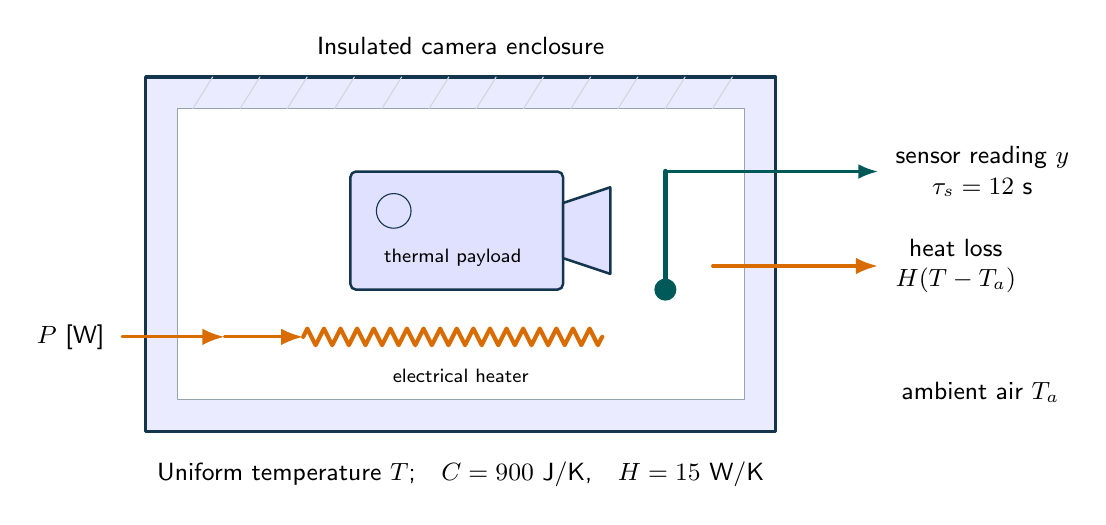
\begin{tikzpicture}[
font=\sffamily\small,>=Latex,line cap=round,line join=round,
wall/.style={draw=ink,line width=1.2pt,fill=blue!5},
water/.style={fill=cyan!25,draw=none},
metal/.style={draw=ink,fill=blue!12,line width=.9pt},
flow/.style={->,draw=blue!65!black,line width=1.2pt},
heat/.style={->,draw=orange!85!black,line width=1.1pt},
measure/.style={->,draw=teal!70!black,line width=.9pt},
dim/.style={<->,draw=ink!65,line width=.6pt},
spring/.style={draw=ink,decorate,decoration={coil,aspect=.5,segment length=4pt,amplitude=3pt}},
wire/.style={draw=ink,line width=1pt},
lab/.style={align=center,font=\sffamily\small},
smalllab/.style={align=center,font=\sffamily\scriptsize}]

\fill[blue!8] (1,0) rectangle (9,4.5);
\fill[white] (1.4,.4) rectangle (8.6,4.1);
\draw[ink,line width=1.2pt] (1,0) rectangle (9,4.5);
\draw[ink!45] (1.4,.4) rectangle (8.6,4.1);
\foreach \x in {1.6,2.2,...,8.2}{\draw[ink!20](\x,4.1)--++(.25,.4);}
\node[lab]at(5,4.9){Insulated camera enclosure};
\draw[metal,rounded corners=2pt](3.6,1.8)rectangle(6.3,3.3);
\draw[metal](6.3,2.2)--(6.9,2)--(6.9,3.1)--(6.3,2.9)--cycle;
\draw[ink](4.15,2.8)circle(.22);
\node[smalllab]at(4.9,2.2){thermal payload};
\draw[heat](2,1.2)--(3,1.2);
\draw[orange!85!black,line width=1.5pt,decorate,decoration={zigzag,segment length=6pt,amplitude=3pt}](3,1.2)--(6.8,1.2);
\node[lab,anchor=east]at(.6,1.2){$P$ [W]};
\draw[heat](.7,1.2)--(2,1.2);
\node[smalllab]at(5,.7){electrical heater};
\draw[teal!70!black,line width=2pt](7.6,1.8)--(7.6,3.3);
\fill[teal!70!black](7.6,1.8)circle(.14);
\draw[measure](7.6,3.3)--(10.3,3.3);
\node[lab,anchor=west]at(10.4,3.3){sensor reading $y$\\$\tau_s=12$ s};
\draw[heat](8.2,2.1)--(10.3,2.1);
\node[lab,anchor=west]at(10.4,2.1){heat loss\\$H(T-T_a)$};
\node[lab]at(11.6,.5){ambient air $T_a$};
\node[lab]at(5,-.55){Uniform temperature $T$;\quad $C=900$ J/K,\quad $H=15$ W/K};
\end{tikzpicture}
}\par{\small Cutaway of a lumped thermal enclosure. Orange arrows carry heat; the probe measures a lagged temperature. The drawing fixes the energy boundary, not a real device geometry.}\end{center}
\begin{enumerate}
\item An enclosure has thermal capacitance $C=900$ J/K and conductance $H=15$ W/K. With constant ambient temperature, define $x=T-T_a$ and derive the balance from heat input $P$ to $x$. Give the units of every term and the zero-state transfer function.
\item Keep $C=900$ J/K but increase $H$ from 15 to 20 W/K. Compare the time constants and the steady rises for 40 W. Find the heater power required to maintain a 3 K rise in each design.
\item A redesigned box must maintain a 3 K rise with at most 45 W and have thermal time constant no greater than 45 s. Keep $C=900$ J/K and vary only $H$. Derive both constraints and decide whether any design is feasible.
\end{enumerate}
\vfill{\small\textbf{Submission.} Show the model, intermediate reasoning, units and a conclusion addressing the stated requirements.}

\newpage
\task{2}{A reassuring sensor reading can hide stored heat}
The nominal box receives a 40 W step from ambient. Its temperature sensor has its own state and a 12 s lag. Evaluate the largest disagreement between the payload and its indicated temperature.
\begin{enumerate}
\item A sensor obeys $12\dot y=x-y$, initially $y=0$. For the 40 W heat step, derive $Y/P$, $y(t)$ and both initial slopes. Explain the different relative degrees.
\item For the previous step, find the time and magnitude of the largest positive error $e=x-y$. Verify the error is zero initially and vanishes as time tends to infinity.
\item Suppose a limit is checked using only the indicated rise $y$. Find the smallest constant allowance $\Delta$ such that $x(t)\le y(t)+\Delta$ for this particular step. Explain why that allowance is not a universal safety margin.
\end{enumerate}
\vfill{\small\textbf{Submission.} Show the model, intermediate reasoning, units and a conclusion addressing the stated requirements.}

\newpage
\task{3}{A heating pulse with a finite energy budget}
The heater can operate at 40 W for only one minute. A 2 K target is desired, followed by passive cooling. Reconcile the continuous-heating prediction with the pulse experiment.
\begin{center}\resizebox{\ifdim\width>.98\linewidth.98\linewidth\else\width\fi}{!}{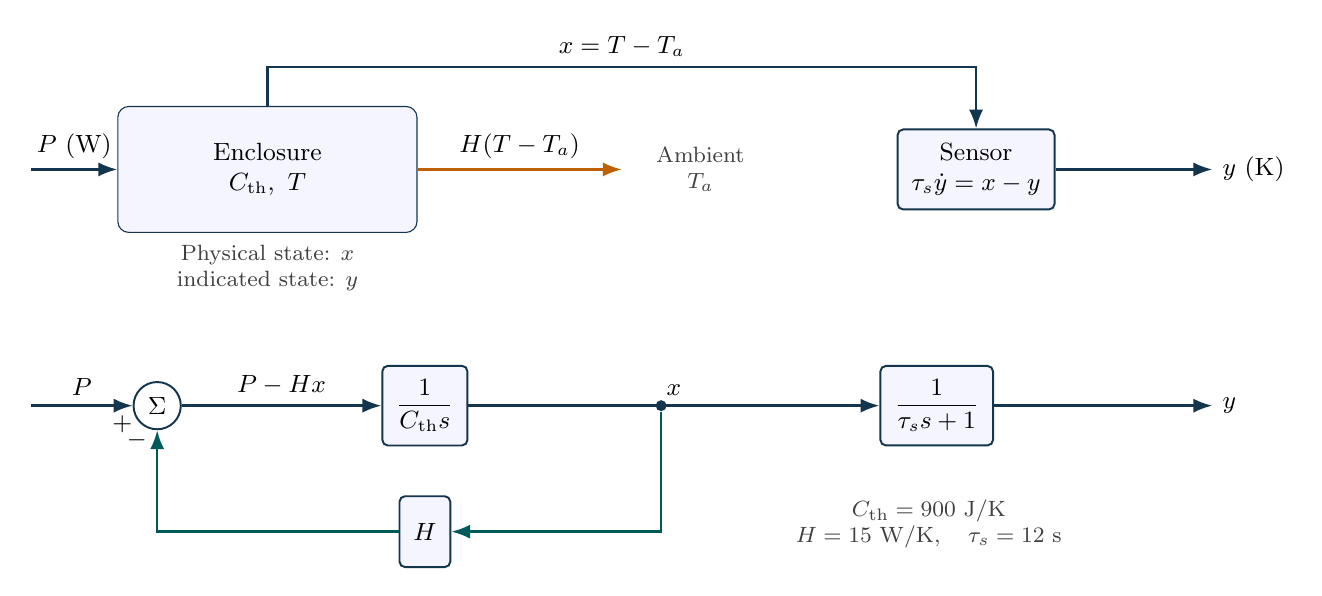
\begin{tikzpicture}[x=1cm,y=1cm,>=Latex,font=\small,
block/.style={draw=ink,fill=blue!4,rounded corners=2pt,minimum height=9mm,align=center,line width=.7pt,inner sep=5pt},
sum/.style={circle,draw=ink,fill=white,minimum size=6mm,inner sep=0pt,line width=.7pt},
sig/.style={->,draw=ink,line width=.85pt},
fb/.style={->,draw=teal!70!black,line width=.85pt},
dist/.style={->,draw=orange!75!black,line width=.85pt},
tap/.style={circle,fill=ink,inner sep=1.4pt},
note/.style={font=\footnotesize,align=center,text=black!75}]

\node[draw=ink,fill=blue!4,rounded corners,minimum width=38mm,minimum height=16mm,align=center](en)at(3,2.5){Enclosure\\$C_{\mathrm{th}},\ T$};
\draw[sig](0,2.5)--node[above]{$P$ (W)}(en.west);
\draw[dist](en.east)--node[above]{$H(T-T_a)$}(7.5,2.5);
\node[note]at(8.5,2.5){Ambient\\$T_a$};
\node[block](sensor)at(12,2.5){Sensor\\$\tau_s\dot y=x-y$};
\draw[sig](en.north)--(3,3.8)--node[above]{$x=T-T_a$}(12,3.8)--(sensor.north);
\draw[sig](sensor.east)--(15,2.5)node[right]{$y$ (K)};
\node[note]at(3,1.25){Physical state: $x$\\indicated state: $y$};
\node[sum](s)at(1.6,-.5){$\Sigma$};
\node[block](int)at(5,-.5){$\dfrac{1}{C_{\mathrm{th}}s}$};
\node[tap](xt)at(8,-.5){};
\node[block](gs)at(11.5,-.5){$\dfrac{1}{\tau_s s+1}$};
\draw[sig](0,-.5)--node[above]{$P$}node[pos=.9,below]{$+$}(s);
\draw[sig](s)--node[above]{$P-Hx$}(int);
\draw[sig](int)--node[above]{$x$}(gs);
\draw[sig](gs)--(15,-.5)node[right]{$y$};
\node[block](h)at(5,-2.1){$H$};
\draw[fb](xt)--(8,-2.1)--(h);
\draw[fb](h)--(1.6,-2.1)--node[pos=.9,left]{$-$}(s);
\node[note]at(11.4,-2){$C_{\mathrm{th}}=900\ \mathrm{J/K}$\\$H=15\ \mathrm{W/K},\quad\tau_s=12\ \mathrm{s}$};

\end{tikzpicture}
}\par{\small Thermal storage, heat leakage and sensor dynamics are separate elements. The lower loop implements the energy balance, not an added temperature controller.}\end{center}
\begin{enumerate}
\item Starting at ambient, apply $P=40$ W. Find the equilibrium rise, initial slope and time to reach a rise of 2 K. Is a 3 K target reachable with this constant input?
\item Apply 40 W for 60 s and then switch the heater off. Derive the physical temperature rise before and after switch-off, and determine the additional cooling time needed to fall to 0.5 K.
\item Compute supplied energy, stored incremental energy and heat lost by the switch-off time. Use the balance to explain why the pulse cannot reach the 2 K target even though continuous heating can.
\end{enumerate}
\vfill{\small\textbf{Submission.} Show the model, intermediate reasoning, units and a conclusion addressing the stated requirements.}

\newpage
\task{4}{Identifying a thermal process through an imperfect instrument}
A synthetic characterization record is available, but the instrument may have unmodeled lag. Assess which parameter conclusions survive that uncertainty and whether inverse filtering fixes the problem.
\begin{enumerate}
\item A deliberately synthetic test gives a 3 K equilibrium rise for a 36 W step. A direct physical-state measurement reaches $1-e^{-1}$ of its final value after 75 s. Identify $H$ and $C$. Explain what changes if the dynamic observation comes from an unmodeled slow sensor.
\item An idealized inverse sensor uses $\hat x_k=y_k+12(y_k-y_{k-1})/\Delta t$. For $\Delta t=1$ s and independent sensor errors of standard deviation 0.02 K, calculate the standard deviation in $\hat x$. Explain the consequence of reducing the sampling interval.
\item Design a two-stage identification and validation protocol that distinguishes heat leakage from storage and sensor lag. State which conclusions cannot be obtained from the quoted equilibrium and fraction-crossing observations alone.
\end{enumerate}
\vfill{\small\textbf{Submission.} Show the model, intermediate reasoning, units and a conclusion addressing the stated requirements.}

\newpage
\task{5}{A warm start during an ambient-temperature change}
Warm initial conditions and external heating act through different terms of the same balance. Keep the distinction between absolute temperature deviation and rise above the current ambient.
\begin{enumerate}
\item Use absolute temperatures and a 12 s sensor. Derive the transfers from heater power and ambient-temperature deviation to measured temperature. Evaluate the final measured change caused by a 30 W power increment and a simultaneous 2 K ambient increase.
\item At switch-on the enclosure rise is 1 K, the sensor indicates 0 K, and power becomes 40 W. Derive $x(t)$ and $y(t)$ for the nominal parameters. State why multiplying a transfer function by $40/s$ alone is insufficient.
\item Combine the two effects: use absolute deviations with $\Delta T(0)=1$ K, $y(0)=0$, a 30 W heater increment and a simultaneous 2 K ambient increment. Derive $x(t)=\Delta T(t)$ and the measured deviation $y(t)$, and check initial and final values.
\end{enumerate}
\vfill{\small\textbf{Submission.} Show the model, intermediate reasoning, units and a conclusion addressing the stated requirements.}

\end{document}
